Dieses Experiment dient als Vergleich zum Vorangegangenen. Die Auswirkung die die Anzahl der Roboter hat, soll hiermit untersucht werden. 

\textbf{Aufbau des Experiments}
\begin{figure}[H]
    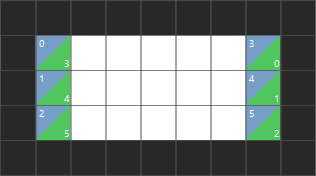
\includegraphics[height=40mm]{images/3vs3.png}
    \centering
    \caption{Aufbau für die enge Vorbeifahrt zweier Gruppen, bestehend aus jeweils drei Agenten}
    \label{fig:3x3}
\end{figure}
Die Karte für dieses Experiment ist sieben mal drei Felder groß. Es stehen sich zwei Gruppen aus jeweils drei Agenten gegenüber. Wie in Abbildung \ref{fig:3x3} zu erkennen, befindet sich zwischen den beiden Gruppen ein Block aus fünf mal drei freien Feldern.